\documentclass[a4paper, 12pt]{article}


\usepackage{graphicx}
\usepackage{xcolor}
\usepackage{mdframed}
\usepackage { amsmath , amssymb , amsthm }
\usepackage[T2A]{fontenc}
\usepackage[utf8]{inputenc}
\usepackage[english,russian]{babel}

\graphicspath{{img/}}
\DeclareGraphicsExtensions{.pdf,.png,.jpg}


\title{Математический анализ}
\author{Алла Владимировавна Устюжанова}
\date{\today}

\begin{document}
\sffamily
\maketitle
(323Л или 407Л для ответов по вопросам в 17:30 по четвергам)
\section*{Лекция 1}

\section{Глава 1. Введение. }
\subsection{Параграф 1: Множества операции над множествами}
Кванторы:
\[
	\forall \quad \exists
\]
Множество -- это совокупность каких-либо предметов(элементов).
\[
	A \quad B , \\\quad
	x \in A,\\ \quad
	x \not\in B,	\\\quad
	A \in B\\
\]
Операции: \\
1. $ A \cup B $ -- те множество каждый элемент которого принадлежит хотябы одному из множеств A или B \[
	A \cup B = \{x:x \in A \quad or \quad x \in B\}	
\]
2. $ A \cap B $ -- это множество каждый элемент которого принадлежит одновременне и A и B \[
	 A \cap B = \{x: x\in A \quad and \quad x \in B\}	
\]
3. $ A \setminus B $ -- (Разность)\[
	A \setminus B = \{x: x\in A \quad but \quad x\not\in B\}	
\]
4. $ CA \quad\bar{A} $ -- (Дополнение) \[
	CA = \bar{A} - S\setminus A	
\]


Виды множеств:\\
$ N \subset Z \subset Q \subset R \subset C $\\

\subsection{Абсолютная величина}
\[
	|x| = \{x \quad x \geq 0 \quad or \quad -x \quad x\leq 0\}	
\]
\subsubsection*{Свойства:}
1. Неравенство треугольника \[
 |x+y| = |x| + |y|	
\]
\begin{mdframed}[backgroundcolor=blue!20] 
       Док-во: пусть $  x+y \geq 0\Rightarrow |x+y| = x+y=|x|+|y|$\\
       Док-во: пусть $  x+y < 0\Rightarrow |x+y| = x+(-y)<|x|+|y|$
    \end{mdframed}

2. $  |x - y|= |x| - |y|$ если $ |x| > |y| $
3. $ |xyz| = |x||y||z| $
4. $ \left| \frac{x}{y}\right| =  \frac{|x|}{|y|}$
sgn x = $ \{ 1 \quad x>0 \quad 0 \quad x=0\} $\\

\subsubsection*{Бином Ньютона:}
\[
	\left( a + b\right)^n = a^n + C_n^1 a^{n-1}b +...+b^n	
\]
\[
	C_n^k = \frac{n!}{(n-k)!k!}	
\]

\[
	n! = 1\cdot 2 \cdot 3 \cdot ... \cdot n	
\]
\[
	0! = 1	
\]


\subsubsection*{Треугольник Паскаля:}
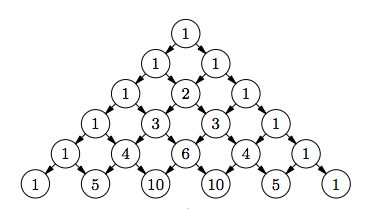
\includegraphics{Pascal_triangle}

\subsubsection{Упражнения}
1. $ A=\{1,2,3\} \quad B=\{2,3,4,5\} \quad A\cup B ? $\\
2. $ A = \{x \in N: \quad 2 < x < 4\} \quad B = \{x \in N: \quad 2 < x < 4\} \quad C = \{x \in N: \quad 2 < x < 4\} \quad B\cup C ?, A\cap B\cap C,A\cup B\cup C \quad ?$\\
3. $ (A\cap B)\cup C = (A\cup C)\cap(B\cup C)? $\\
4. $ (A \setminus B)\cap C = (A\cap C)\setminus (B\cap C) $\\
5. $ \left( 1-x\right)^5 = ?\\$
6. $ \left(\frac{2}{x} + 3 \sqrt[]{x} \right)^4 $\\
\section{Глава 2. Предел и непрерывность.}
\begin{mdframed}[backgroundcolor=blue!20] 
       Курс: Мат анализ (фтф:ИВТ)\\
       код слово: предел
    \end{mdframed}
\subsection{Параграф 1. Предел псоледовательности}
Предел -- пусть каждому натуральному числу N по некоторому закону поставленно в соответствие действительное число $ x_n $ тогда говорят что определена числовая последовательность $ \{x\} = \{x_1,x_2,....,x_n,...\} $ \\
Число a называется пределом последовательности $ \{x_n\}  $ если для всякого действительного числа $ \epsilon  > 0$ найдется зависящее от $ \epsilon $ число такое что выполняется неравенство $ |x_n - a| < \epsilon  $ для всех натуральных чисел $ n > n_0 $.  \\
\\Обозначение:\\
\[
	\lim_{n\to 0} x_n  = a \quad(x_n \to a \quad n \to \inf)	
\]
 
 \[
 	\lim_{n\to 0} x_n = a \Leftrightarrow  \quad \forall \epsilon > 0 \quad \exists n_0 = n_0(\epsilon): \forall n > n_0 \quad |x_n -a| < \epsilon
 \]
\begin{mdframed}[backgroundcolor=blue!20] 
       Пример: $  \lim_{n\to 0} \frac{1}{n}=0 $\\
       $|\frac{1}{n}| < \epsilon, \quad \frac{1}{n} < \epsilon, \quad n > \frac{1}{\epsilon}, \quad n_0 = \left[\frac{1}{\epsilon}\right] + 1 \quad \forall \epsilon>0 $\\
       чтд.
    \end{mdframed}
Произвольный интервал $ AB $ содержащий точку С называется окресностью это точки\\
\[
	\cup(C)	
\]

Эпсилон окресность:\\
\[
	\cup(\epsilon)	\quad {\cup_\epsilon}(\epsilon) = \dot\cup_\epsilon(\epsilon) \setminus {c}
\]
Число(точка) а является пределом последовательности $ x_n $
если для любого эпсилон больше нуля найдется число $ n_0 $ такое что все точки $ x_n $ с индексами $  n > n_0$ попадут в $ \epsilon $окресность точки а. Вне любой окресности точки а имеется конечная или пустое множество точек $ x_n $.


\section*{Лекция 2}
%дописать T1.

\begin{mdframed}[backgroundcolor=blue!20] 
       Теорема 1: Если последовательность $  {x_n}$имеет конечный предел, то он единственный.\\
       Док-во: ${x_n}$ имеет два различных предела а и b.\\ расмотрим окресность cd, тк  $  x_n \to a$ , то ляляля, тогда в интервале не может содержаться бесконечное число элементов, те последовательность $  {x_n}$ не может стремится к b.\\ \\
       Теорема 2: Если последовательность сходится(имеет прредел), то она ограничена.
       Опр: если $ |x_n| \leq M, \quad  M = const$ ,то $  {x_n}$ наз ограниченной\\ \\ 
          Теорема 3(придельный переход в неравенствах):\\
         а) Если $  x_n \to a, \quad y_n \to b, \quad a < b$, то $  \exists n_0^\forall n>n_0 \quad x_n < y_n$\\
         б) Если $  x_n \to a, \quad y_n \to b,\quad x_n \leq y_n \quad \forall n, $ то $ a \leq b $ \\ \\ 
       Теорема 4(принцiп "двух милиционеров"):\\
       Если $  x_n \to a, \quad y_n \to a \quad and \quad x_n \leq z_n \leq y_n \quad \forall n \in N \quad then \quad z_n \to a$ \\ \\
       Теорема 5(Арифметические свойства приделов):\\
       1) $ \lim_{n\to inf} c = c, \quad c = const  $\\
       2) $  if \quad \exists \quad ending \quad \lim_{n\to inf} x_n = a, \quad \lim_{n\to inf} y_n = b \quad then \quad  $ существуют приделы их суммы, разности , произведения, частного($  b \neq 0$):\\
       	\[a)   \lim_{n\to inf} (x_n \pm y_n) = a + b\] 
       	\[b)   \lim_{n\to inf} (x_n y_n) = ab \]
       \[	c)   \lim_{n\to inf} \left(\frac{x_n}{y_n}\right) = \frac{a}{b},\quad where \quad b\neq 0 \]

       Определение: $ {x_n} $ называется бесконечно малой если предел последовательности равен 0\\
       
       Определение: $ {y_n} $ называется бесконечно большой если предел последовательности равен бесконечности \[
       	\forall \epsilon > 0 \quad \exists n_0 : \quad \forall n > n_0 \quad |y_n| > \epsilon
       \]
       Свойства:\\
       1) произведение бесконечно малой на ограниченное является бесконечно малой\\
    \end{mdframed}

\subsection{Параграф 2. Предел функции}
-- Функцией называется закон по которому каждому x из некоторово множества D соответствует единственное значение y из множества E\\
\[
 y = f(x)	
\]
\[
 f: D \to E	
\]
где x -- независсимая переменная, аргумент\\
y -- зависимая переменная\\
D -- область определения\\
E -- область значения\\


       Определение предела функции\\
       1. по Коши\' (с помощью окресности):
       \[
        \lim_{x\to 0} f(x)  = A \quad \Leftrightarrow \quad \forall \cup_\epsilon (A) \quad \exists \cup_\epsilon (x_0)  \quad \forall x \in \cup_\epsilon (x_0) \quad \Rightarrow \quad f(x) \in \cup_\epsilon (A)	
        \] 

        с помощью неравенства:\\$
        a) x_0, A - ending \quad \lim_{x\to x_0} f(x) = (A) \Leftrightarrow \quad \forall \epsilon > 0 \quad \exists b > 0: \quad 0 < |x-x_0| < b \Rightarrow \quad |f(x) - A| < \epsilon 	
        $\\
        $
        b)x_0 - ending, A = +inf \quad \lim_{x\to x_0} f(x) = +inf \Leftrightarrow \quad \forall \epsilon > 0 \quad \exists \delta > 0 : \quad |x-x_0|< \delta \Rightarrow \quad f(x) > \epsilon 	
        $\\
        $
        c)x_0 - ending, A = -inf \quad \lim_{x\to x_0} f(x) = -inf \Leftrightarrow \quad \forall \epsilon > 0 \quad \exists \delta > 0 : \quad |x-x_0|< \delta \Rightarrow \quad f(x) < - \epsilon	
        $\\
        $
        d)x_0 - ending, A = inf \quad \lim_{x\to x_0} f(x) = inf \Leftrightarrow \quad \forall \epsilon > 0 \quad \exists \delta > 0 :\\ |x|> \delta \Rightarrow \quad |f(x)-A| <  \epsilon	
        $

        2) по Гейне(с помощью предела последовательности):\\
        $
        A = \lim_{x\to x_0} f(x) \Leftrightarrow \quad \forall {x_n} \to x_0 \quad n \to inf, \quad {x_n} \neq x_0	
        $\\
        Соответсвующая последовательность значений функции\\ ${f(x_n)} \to A \quad n \to inf$

\begin{mdframed}[backgroundcolor=blue!20] 
       Теорема 1(Арифметические свойства пределов функции): \\
       Пусть существует конечные пределы функции \[
       	\lim_{x\to x_0} f(x) = A, \quad \lim_{x\to x_0} g(x) = B
       \]

       тогда предел суммы(разности) равен пределу суммы(разности)\\
       произведения = произведению\\
       частного = частному\\
       ограниченна в некоторых окресностях точки $ x_0 $\\ \\ 

       Теорема 2 (предельный переход в неравенство):\\
       \[
       		\lim_{x\to x_0} f(x) = A, \quad \lim_{x\to x_0} g(x) = B, \quad \exists \cup(x_0),f(x)<g(x) \quad f(x) \in \cup(x_0)
       \]

       


    \end{mdframed}



\section*{Лекция 3}


Введем понятие сложной функции:\[
  f:X \to Y \quad y = f(x)
\]
\[
  g:Y \to R \quad g(y)
\]
\[
  h:X \to R \quad h(x) = g(f(x))= g \circ f
\]

\begin{mdframed}[backgroundcolor=blue!20] 
       Теорема 3(предел сложной функции):\\
       пусть $ \lim_{x\to x_0} f(x) = y_0, f(x) \neq y_0 ,x \neq x_0  $, $ \exists \lim_{y\to y_0} g(y) = A \Rightarrow \exists \lim_{x\to x_0}h(x) = \lim_{x\to x_0} g(f(x)) = A    $\\

       Теорема 4(критерий Коши):\\
       Функция f(x) имеет придел в точке $ x_0 $  тогда и только тогда выполнения условия $ \forall \epsilon > 0 \quad \exists \epsilon > 0 : \quad \forall x',x'': \quad |x' - x_0|<\epsilon $ \\
       \[
         |f(x') - f(x'')| < \epsilon
       \]

    \end{mdframed}


\subsubsection*{Односторонние пределы}
--\\
Предел с лево($ x \to -0$): 
\[
  A = \lim_{x\to x_0 - 0} f(x) = f(x_0-0) \quad \Leftrightarrow \quad 
\]
\[
  \forall \epsilon > 0 \quad \exists \delta > 0:x_0 - \delta < x < x_0 \quad \Rightarrow \quad |f(x) - A| < \epsilon
\]
Предел с право($ x \to +0) $:
\[
  A = \lim_{x\to x_0 + 0} f(x) = f(x_0+0) \quad \Leftrightarrow \quad 
\]
\[
  \forall \epsilon > 0 \quad \exists \delta > 0:x_0  < x < x_0 + \delta \quad \Rightarrow \quad |f(x) - A| < \epsilon
\]
Замечание:\\ 
1)Функция имеет предел при $ x \to x_0 $, когда существуют левый и правый пределы равные между собой.\\
2)Если $ A = \lim_{x\to x_0} f(x) $ то \[
  f(x) = A + \alpha(x) \quad \alpha(x)\to 0
\]

\subsection{Параграф 3. Замечательные пределы}

1ый замечательный предел:
\[
  \lim_{x\to 0}  \frac{\sin x}{x} = 1
\]
следствие 
\[
  \lim_{x\to x_0} \frac{\sin \alpha(x)}{\alpha (x)} = 1 
\]

2ой замечательный предел
\[
  \lim_{x\to +inf} 1 + \frac{1}{x} = \lim_{x\to -inf}(1 + \frac{1}{x})^x=\lim_{x\to inf}(1 + \frac{1}{x})^x = e\simeq 2.718281828\ldots
\]
следствие \[
  \lim_{\alpha\to 0} (1 + \alpha)^\frac{1}{\alpha} = e 
\]

\subsection{Параграф 4. Непрерывность функции}
-- Функция $ y = f(x) $ называется непрерывной в точке $ x_0 $, если \\
$ \lim_{x\to x_0}f(x) = f(x_0)  $\\

Функция непрерывна на множестве D  если она не прерывна к каждой точке этого множества. 
Если одно из условий непрерывности не выполняется, то функция не является непрерывной в этой точке.\\

Точка разрыва -- это когда $f(x)$ определена проколотой окресностью этой точки и не является непрерывной в точке $ x_0 $\\

\subsubsection{Классификация точек разрыва}
a) $ x_0 $ называется точкой устранимого разрыва  $ f(x) $, если существует предел функции при $ x\to x_0 $(конечный предел), но функция либо не определена в $ x_0 $, либо значение предела не совпадает со значением функции\\
b) $ x_0 $ называется точкой разрыва первого рода функции $ f(x) $, если $ \exists  $ют конечные односторонние пределы.\\  
c) $ x_0 $ называется точкой разрыва второго рода, если хотябы один из односторонних пределов не существует или является бесконечным.\\

\newpage
\subsubsection{Основные теоремы о непрерывных функциях}

\begin{mdframed}[backgroundcolor=blue!20] 
      
       Теорема 1\\
       Сумма, разность, произведение, частное(знаменатель не равен нулю) непрерывных функций также являются непрерывной функцией.\\

       Теорема 2(непрерывность сложной функции)\\
       Пусть сложная функция определена в окресности $ x_0 $, пусть функция y = g(x) непрерывна в точке $ x_0 $, внешная функция $ y_0 $=f($ x_0 $) непрерывная в точке $ y_0 $, тогда f(g(x)) непрерывна в $ x_0 $\\

       Теорема 3(о промежуточном значении)\\
       Пусть f(x) непрерывна на AB и на его концах принимает значение разных знаков, тогда существует точка 'c' внутри AB, f(c)=0.\\

       Теорема 4(о макс значении Вейерштрасса):\\
       Функция f(x) непрерывная на AB является оганиченной на этом отрезке и приэтом существует точка x1 из AB такая что x1 максимальное значение функции, также есть точка x2 которая является минимальным значением функции.
    \end{mdframed}

Следствие теоремы 3: Если $ \phi(x)  $ непрерывна на AB, то найдется точка 'c' из интервала AB, $ \phi(x=c) = C $\\
\section*{Лекция 4}
Введем понятие обратной функции:
\[
  y = f(x): D \to E
\]
если каждому y из множества Y ПОСТАВИТЬ В СООТВЕТСТВИЕ ЗНАЧЕНИЕ x из D то получим обратную функцию.
\[
  x = f^{-1}(y)
\]

\newpage
\begin{mdframed}[backgroundcolor=blue!20] 
       Теорема 5(о непрерывности обратной функции)\\
       Пусть $ y = f(x) $ непрерывна, строго возрастает(убывает) на [a,b] $ f(a) = A,\quad f(b)=B \quad  A<B(A>B)$, тогда обратная функция $ x = f^{-1}(y) $ определена на [A,B] непрерывно и является возрастающей(убывающей)\\

       Теорема Элементарные функции\\
       $ y = kx +b;\quad y = x^x; \quad y = \sin x;y = \ln_a x;\quad  y=a^x \ldots $, эти функции непрерывны на всей области определения.   
    \end{mdframed}
    
\subsection{Параграф 5. Сравнение Ассимптотического поведения функции.}
-- это поведение функции вблизи некоторой точки.\\

Пусть $ \alpha (x), \beta (x) $ б.м в окресности точки $ x_0 $, т.е $ \lim_{x\to x_0} \alpha (x)  = \lim_{x\to x_0} \beta (x) = 0$   

Определение:\\
Функция $ \alpha (x) $ называтеся бесконечно малой более высокого порядка чем $ \beta (x) $ если $ \lim_{x\to x_0} \frac{\alpha (x)}{\beta (x)} = 0  $\\
\[
   \alpha (x) = o(\beta (x))
 \] 
o -- 'o' малое(не нуль)\\

Определение:\\
Функция $ \alpha (x) \quad  \beta (x) $ б.м одного порядка если $ \lim_{x\to x_0} \frac{\alpha (x)}{\beta (x)} = A \neq 0 \neq inf $\\
$ \alpha (x)\quad \beta (x) $ назыв эквивалентными б.м огранич при $ x \to x_0 $ если предел отношения равен 1($ \alpha (x) \sim \beta (x): x\to x_0 $) \\

\begin{mdframed}[backgroundcolor=blue!20] 
       Теорема\\
       Если $ \alpha (x)\sim \alpha_1 (x);\beta (x)\sim \beta_1 (x) $ то \[
         \lim_{x\to x_0} \frac{\alpha (x)}{\beta (x)} = \lim_{x\to x_0} \frac{\alpha_1 (x) }{\beta_1 (x)}
       \] 
    \end{mdframed}
    
Таблица эквивалентных б.м при $ x \to x_0 $:
\begin{align}
  \sin x \sim x \\
  \tg x \sim x\\
  \arcsin x \sim x\\
  \arcctg x \sim x\\
  \ln (1+x) \sim x\\
  \frac{a^x - 1}{\ln a} \sim x\\
  \frac{(1+x)^a - 1}{a} \sim x\\
  e^x -1 \sim x
\end{align}

\section{Глава. Дифференциальное исчесление функции одной переменной}
\subsection{Параграф 1. Понятие производной функции}
\begin{align*}
  y = f(x)\\
  \Delta x = x - x_0 \\
  x = x_0 + \Delta x\\
  \Delta y = f(x) - f(x_0) = f(x_0 + \Delta x) - f(x_0)
\end{align*}

Производная -- производная функции в точки $ x_0 $  называется 
\begin{align}
  \lim_{\Delta x\to 0} \frac{\Delta y}{\Delta x} = \frac{d}{dx} f(x) = f'(x)
\end{align}

Левая производная:
\begin{align}
  f_{-}'(x) = f'(x - 0) = \lim_{\Delta x\to 0-0} \frac{\Delta y}{\Delta x} 
\end{align}

Правая производная:
\begin{align}
  f_{+}'(x) = f'(x + 0) = \lim_{\Delta x\to 0+0} \frac{\Delta y}{\Delta x} 
\end{align}

Связь левой и правой производной
\begin{align*}
  \exists f'(x) \Leftrightarrow \exists f_{-}'(x) = f_{+}'(x) = f'(x)
\end{align*}

\subsubsection{интерпретации производной}
1)Геометрическая:\\

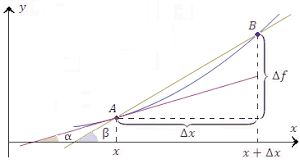
\includegraphics{img/dif.png}\\
$ AB  $ -- секущая(при $ \Delta x  \to 0$ называется касательной) \\
$ \Delta x \to 0 \Rightarrow \beta  \to \alpha  \Rightarrow \quad  \tg \beta  \to \tg \alpha  $\\
$ \tg \beta  =  \frac{\Delta y}{\Delta x}; \quad  \tg \alpha  = f'(x) $\\
$ y_k = f(x_0) + f'(x_0)(x - x_0) $ -- уравнение касательной\\
$ y_n = f(x_0) - \frac{1}{f'(x_0)} - (x - x_0) $ -- уравнение нормали \\

опр. Функция называется дифференцируемой в точку $ x_0 $  если приращение можно представить в виде $ y = A \cdot \Delta x +\alpha (\Delta x) \cdot \Delta x $,  где A незавитсамая переменная($ \Delta x \to 0 $) . 
\[
     \Delta y = A \Delta x + o(\Delta x)
   \]   
   \begin{mdframed}[backgroundcolor=blue!20] 
          Теорема 1(связь между дифференциироваемостью и существованием производной)\\
          Для того чтобу функция $ f(x) $ была дифференциируема в точке $ x_0 $ необходимо чтобы она имела производную в точке $ x_0 $ \\

          Теорема 2(связь между диф и непрерывностью)\\
          Если f(x) диф в точке  $ x_0 $  то она непрерывна в этой точке(обратное не работает)\\
       \end{mdframed}



       
2)Физическая(мгновенная и средняя скорости):\\
\[
  s = f(t) \quad v_m = \frac{f(t + \Delta t) - f(t)}{\Delta t} = \frac{\Delta f}{\Delta x}
\]
-- это скорость изменения функции.

\subsection{Основные правила дифференциирования}

\begin{align}
  \frac{d}{dx} (c) = 0, c = const\\
  \frac{d}{dx} (u \pm v) = u' \pm v'\\
  \frac{d}{dx} (uv) = u'v+u v'\\
  \frac{d}{dx} cu = c u',c=const\\
  \frac{d}{dx} \left(\frac{u}{v}\right) = \frac{u' v - uv'}{v^2}
\end{align}

\textbf{Гиперболические функции:}\\

Гиперболический синус:\\
\[
  \sh x = \frac{e^x-e^{-x}}{2}
\]
Гиперболический косинус:\\
\[
  \ch x = \frac{e^x+e^{-x}}{2}
\]
Гиперболический тангенс и котангенс:\\
\[
  \th x = \frac{\sh x}{\ch x} \quad  \cth x = \frac{1}{\th x}
\]

\subsubsection*{Понятие о частных производных}
\[
  f(x,y)
\]
\[
  f_x' = \frac{\partial f}{\partial x} \quad y=const 
\]
\[
  f_y' = \frac{\partial f}{\partial y} \quad x=const
\]

\subsection{Производная сложной функции}

\begin{align}
  \frac{d}{dx} f(u(x)) = u'(x) \cdot f'(u(x)) 
\end{align}

\subsubsection*{Производная обратной функции}

\begin{align}
  y = f(x),f'(x)\neq 0,\exists x=f^{-1}(y),\Rightarrow x_y' = \frac{1}{y_x'}
\end{align}

\subsubsection{Производная функции заданной в параметрическом виде}

\begin{align*}
  x = f(t) \quad and \quad y = g(t): x' \neq 0 \Rightarrow t = f^{-1}(x) \quad  t'_x = \frac{1}{x'_t}\\
  y = y(x) = y(x(t)) :  y'_x = y'_t  t'_x=y'_t  \frac{1}{x'_t} = \frac{y'_t}{x'_t}\\
\end{align*}


\subsubsection{Дифференциирование функции заданной неявно}

Рассмотрим неявно заданную функцию, т.е когда функця  $ y = y(x)  $ задается равенством вида $ F(x,y) = 0 $.\\
Чтобы найти производную функции заданной неявно нужно диф-вать равенство $ F(x,y) = 0 $ по переменной $ x $ при этом $ y $ считаем функцией от $ x $.\\

\[
        y'_x = \frac{\frac{\partial F}{\partial x}}{\frac{\partial F}{\partial y}} = \frac{F'_x}{F'_y}
      \]      

\subsection{Дифференциал функции}

$ \Delta f = f'(x) \Delta x + o(\Delta x) $\\

Дифференциал функции -- \[
  \Delta f = f'(x) \Delta x
\]
в дальнейшем: $ df = f'(x) dx $\\
следствие:

\[
  f'(x) = \frac{df}{dx}   
 \] 

св-ва(теже что и у производной )+ свойство инвариантности(сохранения формы):\\
1)для первого порядка: $ y(u(x)): dy = y'_x dx=y'_x u'_x dx = y'_u du $ \\
Дифференциал первого порядка функции $ y $  выражается по одной и тойже формуле независимо от того будет ли $ y $ рассматриватся как функция от независимой переменной $ x $ или от зависимой переменной $ u $.\\


\subsubsection{Применение дифференциала в приближенных вычеслениях}

При малом $ \Delta x: \quad \Delta y = dy = f'(x)\Delta x = f(x + \Delta x) - f(x) \simeq f(x) + f'(x)\Delta x $ \\

\subsection{Производные и дифференциалы высших порядков}
Производная от производной функции называется производной второго порядка:\\
\begin{align*}
   y'' = (y')' = y^{(2)}  \\
 ...\\
   y^{(n)} \\
\end{align*}


Дифференциалом второго порядка называется дифференциал от дифференциала, рассматривоемого как функция только от переменной $ x $ (при постоянном $ dx $ ):\\
\begin{align*}
       d^2y = d(dy) = d(f'(x)dx)=(f'(x)dx)'dx=f''(x) dxdx=f''(x) dx^2 \\
      ...\\
       d^ny = f^{(n)}(x) (dx)^{n} 
    \end{align*}
свойства инвариантности дифференциалы высшего порядка не обладает.\\

\subsection{Теоремы о средних значениях}

Опр.\\
$ f(x) $ достигает точки $ x = c $ локальный максимум(минимум) если существует окресность этой точки в которой выполняется: $ f(c) \geq f(x) \quad \forall x \in \cup(c)\quad (f(c) \leq f(x) \quad \forall x \in \cup(c))$, также называется экстремум(extr)\\
\newpage
\begin{mdframed}[backgroundcolor=blue!20] 
       Теорема Ферма(необходимое условие существования extr)\\
       Если $ f(x) $ имеет производную в точку $ c $ и достигает в этой точке локального эктремума то производная в этой точку равна нулю.\[
         f'(c) = 0
       \] 

       Теорема Ролля\\
       Если $ y = f(x) $ на отрезки AB, дифференцируема на этом же промежутке и значение функции на концах совпадают, то существует точка $ \xi  $ т.ч $ f'(x) = 0 $   


    \end{mdframed}

Геометрический смысл:\\
Если выполнены условия теоремы, то на графики функции существует точка $ (\xi,f(\xi))  $ касательная\\ 
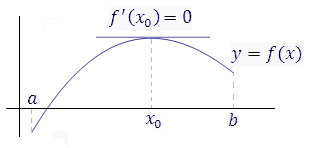
\includegraphics{img/361.png}\\

\begin{mdframed}[backgroundcolor=blue!20] 
       Теорема Коши:\\
       Если f(x),g(x) непрерывны на отрезке AB,f(x) и g(x) дифференцируемы на (a,b),g'(x) $ \neq 0 $, $ \exists \xi \in (a,b), $
       \[
           \frac{f(b)- f(a)}{g(b) - g(a)} = \frac{f'(\xi)}{g'(\xi)}
         \]  

        Теорема Лагранжа\\
        Пусть f(x) непрерывна на AB и дифференциируема на (a,b), тогда существует точка $ \xi \in (a,b): \quad f(b) = f(a) = f'(\xi)(b-a) $\\ 
    \end{mdframed}
\newpage
Геометрический смысл Т. Лагранжа:\\
\quad \quad \quad 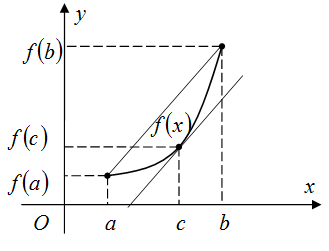
\includegraphics{img/362.png}\\
Следствие -- $ f'(x) = 0 \Rightarrow f(x) = const $ \\

\subsection{Параграф. Правила Лопиталя(раскрытие неопределенности)}
Пусть выполнены условия:\\
1)f(x),g(x) дифференциируемы в окресности точки A, за исключением ,быть может, самой точки A.\\
2)g'(x) $ \neq 0 $ в окресноти A\\
3)$ \lim_{x\to A} \frac{f(x)}{g(x)} = \left\{\frac{0}{0}\right\} \quad  or \quad \left\{\frac{inf}{inf}\right\} $\\
4)$ \exists \lim_{x\to a} \frac{f'(x)}{g'(x)} = A $\\
\[
  \Rightarrow \exists \lim_{x\to a} \frac{f(x)}{g(x)} = \lim_{x\to a} \frac{f'(x)}{g'(x)} = A
\]


Упр. $ \lim_{x\to 0} \frac{x^2 \cos(\frac{1}{x})}{\sin x} $

\newpage
\subsection{Параграф. Формула Тейлора.}
Задача: представить функцию f(x) в некоторой окресности точки A в виде многочлена относительно разности $ x - a $ (разложить по степеням).\\

Пусть f(x) имеет производную до n-ого порядка включительно,\\
Опр.
\[
    f(x) = f(a) + f'(a)(x-a) + \frac{f''(a)}{2!}(x-a)^2 + \ldots + \frac{f^{(n)}(a)}{n!}(x-a)^n + r_n(x)
  \]  

\begin{mdframed}[backgroundcolor=blue!20] 
       Локальная Теорема Тейлора\\
       Если f(x) - непрерывно-дифференцииррованна n раз в окресности A\\($ f(x),f'(x),\ldots,f^{(n)}(x) $-- непрерывно дифференциируема ),то $ r_n(x) = o((x-a)^n) $, записываем в форме Пеано.\\
    \end{mdframed}
    
Формы записи остатка по Коши и Лагранжу:\\
\begin{align*}
   r_n(x) = \frac{f^{(n+1)}(\xi)}{n!}(x-\xi)^n(x-a) \\
   r_n(x) = \frac{f^{(n+1)}(\xi)}{(n+1)}(x-a)^{n+1}\\
 \end{align*}
\textbf{Замечания(формула Маклорена)} -- если в формуле Тейлора вместо $ a $ взять нуль\\
\[
   f(x) = f(0) + f'(0)(x) + \frac{f''(0)}{2!}(x)^2 + \ldots + \frac{f^{(n)}(0)}{n!}(x)^n + r_n(x)
\] 

\subsection{Параграф. Признаки монотонности}

Опр. $ x_1 < x_2, \quad f(x) $ называется возрастающей если $ f(x_1)< f(x_2) $, неубывающая $ f(x_1) \leq f(x_2) $, убывающей $ f(x_1) > f(x_2) $, невозрастающей $ f(x_1) \geq f(x_2) $ \\
Во всех случаях функция называется монотонной(в 1 и 3 строго монотонной).\\  

\begin{mdframed}[backgroundcolor=blue!20] 
       Теорема(Признак монотонности функции)\\
       $ f(x) $- дифференцируема на AB и $ f'(x) > 0(f'(x) < 0):\forall x \in AB $, тогда $ f(x) $ возрастает(убывает) на AB.\\  
    \end{mdframed}
    
\textbf{Правило исследования на возрастание(убывание)}\\
1) находим точки в которых $ f'(x) = 0 $  или несуществует, эти точки называются критическими точками первого рода, они разбивают область определения  на интервалы монотонности\\
2) исследуем знак производной на каждом интервале\\
3) определяем, возрастает или убывает\\

\begin{mdframed}[backgroundcolor=blue!20] 
       
       Теорема(Первый достаточный признак существования экстремума)\\
       f(x) непрерывна в некоторой окресности точки $ x_0 $ и дифференциируема в каждой её точке за исключением быть может точки $ x_0 $. Если при переходе через $ x_0 $ производная меняет знак, то точки $ x_0 $ точка экстремума.\\ 

       Теорема(Второй достаточный признак существования экстремума)\\
       Пусть в окресности $ x_0 $ $ f(x) $ непрерывно дифференцируема $ (n+1) $ раз ($ f'(x_0)= f''(x_0)=\ldots =f^{(n)}(x_0)= 0 \quad f^{(n+1)}(x_0) \neq 0 $ ). Тогда если (n+1) нечетное число - в $ x_0 $ нет экстремума, четное - есть экстремум, причем если $ f^{(n+1)}(x_0) <(>) 0: x_0 - max(min)$     
    \end{mdframed}

Упр. Доказать общий случай.

\subsection{Параграф. Выпуклость и вогнутость прямой, точки перегиба}
График дифференциируемой функции y = f(x) называется выпуклым(вверх) на интервале AB если графика на этом промежутке расположен ниже косательной, проведенной к графику этой функции в любой точки $ x \in (a,b) $, если график расположен выше касательной то его называют вогнутым(выпуклым вниз).\\
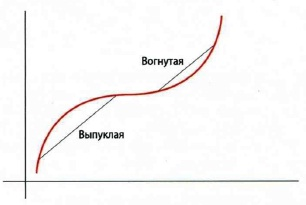
\includegraphics{img/101.jpg}\\

Точка $ (x_0,f(x_0)) $ графика функции y = f(x) называется точкой перегиба если она разделяет вогнутую и выпуклую части графика.\\  

\begin{mdframed}[backgroundcolor=blue!20] 
       Теорема(необходимый и достаточный признак выпуклости и вогнутости)\\
       Пусть f(x) дважды непрерывно дифференциируема на интервале AB , тогда график функции выпуклый(вогнутый) когда\\ $ f''(x) \leq 0(f''(x) \geq 0) \quad \forall x \in (a,b)$ \\

       Теорема(необходимый признак существования точки перегиба)\\
       Если точка $ x_0 $  - точка перегиба дважды непрерывно дифференциируемой функции f(x) то $ f''(x_0) = 0 $  
    \end{mdframed}

Замечание: функция может иметь точку перегиба и при $ x = x_0 $ который $ f'' $  не существует и поэтому возможными точками перегиба являются точки, в которых вторая проихводная равна нулю или не существует. Такие точки называются критическими точками второго рода.\\

\begin{mdframed}[backgroundcolor=blue!20] 
       Теорема(достаточный признак существования точки перегиба)\\
       Пусть f(x) определена в окресности критическойточки второго рода $ x_0 $ и дважды непрерывно дифференциируема хотябы в проколотой окресности точки $ x_0 $. Если $ f''(x) $ меняет знак при переходе $ x_0 $, то точка   $ x_0 $ - точка перегиба.   
    \end{mdframed}
\newpage
\subsection{Параграф. Асимптоты графиков функций}
Прямая $ L: Ax+By +c = 0 $ называется асимптотой графика функции $ y=f(x) $  если растояние $ d $ от точки $ M(x,f(x)) $ до прямой стремится к нулю при неограниченном возрастании модуля $ |f(x)| $  \\ \\
Если $ B = 0 \quad \Rightarrow \quad  x=a $ - вертикальная\\
Если $ B \neq 0 \quad \Rightarrow \quad  y = kx + b$ - наклонная \\
Если $ k = 0 \quad \Rightarrow \quad y=b $ - горизонтальная   \\

\begin{mdframed}[backgroundcolor=blue!20] 
       Теорема 1\\
       Прямая $ x = a $ является вертикальной асимптотой когда выполняется хотябы одно из соотношений:
       \begin{align*}
          \lim_{x\to a-0} f(x) = \pm inf\\
          \lim_{x\to a+0} f(x) = \pm inf
        \end{align*}

        Теорема 2\\
        Прямая $ y = kx+b $ является наклонной асимптотой $ y = f() $ когда существуют конечные пределы:
        \begin{align*}
            k = \lim_{x\to \pm inf} \frac{f(x)}{x}\\
            b = \lim_{x\to \pm inf} (f(x) - kx)
          \end{align*}
    \end{mdframed}

\subsection{Параграф. План полного исследования функции и построение ее графика}
 
1) найти область определения функции\\
2) является ли функция четной(нечетной), переодической\\
3) асимптоты, точки разрыва\\
4) найти промежутки возростания, убывания, экстремумы(с помощью производной первого порядка)\\
5) найти промежутки вогнутости,выпуклости,точки перегиба(с помощью производной второго порядка)\\
6) построить график(для уточнения графика нужно найти точки пересечения с осями координат)\\

(только 8 задание из инд. зад)

\section{Глава. Интегрирование функций одной переменной}

\subsection{Параграф. Неопределенный интеграл и его свойства}

Опр. $ F(x) $ -- называется первообразной для $ f(x) $ на (a,b) если $ F'(x) = f(x) $.\\
Замечание: Если $ F(x) $ - первообразная для $ f(x) $, то $ F(x) + c  $ - тоже\\      
 \begin{mdframed}[backgroundcolor=blue!20] 
        Теорема 1\\
        Если $ F_1(x) \quad F_2(x) $ - первообразные для $ f(x) $,то $ F_1(x)-f_2(x) = const $   
     \end{mdframed}

Опр. Множество всех первообразных для f(x) называется неопределенным интегралом от функции f(x)
\[
  \int_{}^{}\left(f(x)\right)dx = F(x) +c
\]

Нахождение первообразной называется интегрированием.\\

Таблица интегралов:

\begin{align}
  \int_{}^{}\left(x^\alpha\right) dx = \frac{x^{\alpha +1}}{\alpha +1} + c \quad a \neq 1\\ 
  \int_{}^{}\left(\frac{1}{x}\right)dx = \ln |x| +c\\
  \int_{}^{}\left(\sin x\right)dx = - \cos x +c\\
  \int_{}^{}\left(\cos x\right)dx = \sin x + c \\
  \int_{}^{}\left(\frac{1}{\cos^2 x}\right)dx = \tg x +c \\
  \int_{}^{}\left(\frac{1}{\sin^2 x}\right)dx = \ctg x + c\\
  \int_{}^{}\left(e^x\right)dx = e^x + c\\
  \int_{}^{}\left(a^x\right)dx = \frac{a^x}{\ln a} + c\\
  \int_{}^{}\left(\frac{1}{1+x^2}\right)dx = \arctg x + c \\
  \int_{}^{}\left(\frac{1}{\sqrt[]{1-x^2}}\right)dx = \arcsin x + c \\
  \int_{}^{}\left(\frac{1}{a^2 + x^2}\right)dx = \frac{1}{a}\arctg \frac{x}{a} + c\\
  \int_{}^{}\left(\frac{1}{\sqrt[]{a^2 - x^2}}\right)dx = \arcsin \frac{x}{a} + c\\
  \int_{}^{}\left(\frac{1}{a^2 - x^2}\right)dx = \frac{1}{2a}\ln \frac{|a+x|}{|a-x|} +c\\
  \ldots
\end{align}




Основные свойтсва неопределенного интеграла:\\
1) операция интегрирования является обратной к дифференциированию\\
2) интеграл суммы равен сумме интегралов\\
3) константу можно вынести из под знака интеграла\\

\subsection{Параграф. Формула замены переменной под знаком интеграла}
$ x = \phi (t) $ - монотонная и имеет непрерывную производную\\
$ f(x) $ - непрерывна на интервале принадлежащем области значения функции $ x = \phi (t) $, т.е $ f(\phi (t)) $ -- слож функция:
\[
      \int_{}^{}\left(f(x)\right)dx = \begin{vmatrix}
    x = \phi (t)\\
    dx = \phi' (t) dt
  \end{vmatrix} = \int_{}^{}\left(f(\phi (t))\phi'(t)\right)dt 
\]    


\subsection{Параграф. Формула интегрирования по частям}

Пусь $ u(x),f(x) $ -  дифференциируемые  функции, \[
  d(uv) = u dv + v du, \quad \int_{}^{}\left(\right)d(uv) = uv 
\]
тогда: \[
  \int_{}^{}\left(u\right)dv = u v - \int_{}^{}\left(v\right)du 
\]
\[
  \int_{}^{}\left(u(x)v'(x)\right)dx = u(x)v(x) - \int_{}^{}\left(u'(x)v(x)\right)dx 
\]

$ P_n(x) $ - многочлен степени n\\
\[
   1)P_n(x)\cdot (\sin x;\cos x;e^x;a^x)dx: \quad u = P_n(x) \quad dv = (\sin x;\cos x;e^x;a^x)dx
 \] 

\[
  2)\int_{}^{}\left(P_n(x)\begin{Bmatrix}
    \ln x \\
    arctg x\\
    \arcsin x
  \end{Bmatrix}\right)dx: \quad u = \begin{Bmatrix}
    \ln x \\
    arctg x\\
    \arcsin x
  \end{Bmatrix} \quad  
\]

\subsection{Какое-то кол-во пропущенных параграфов}

.................................


\subsection{Параграф. Интегрирования параметрических функций}

\[
   1)\int_{}^{}\left(R(\sin x,\cos x)\right)dx
\]
Данный интеграл сводится к интегралу от рациональной дроби с помощью универсальной подстановки
\begin{align*}
  \tg \frac{x}{2} = t\\
  \frac{x}{2} = \arctg t \quad x = 2\arctg t\\
  dx = \frac{1}{1 + x^2} dt\\
  \sin x = \frac{2t}{1 + t^2} \quad  \cos x = \frac{1-t^2}{1+t^2}\\
  \int_{}^{}\left(R(\sin x,\cos x)\right)dx = \int_{}^{}\left(R\left(\frac{2t}{1 + t^2},\frac{1-t^2}{1+t^2}\right)\right)\frac{2}{1+t^2}dt 
\end{align*}

Частные случаи:\\
a) Если $ R(-\sin x,\cos x) = -R(\sin x, \cos x), \quad R(,) $ является нечетной относительно синуса x
\[
   \Rightarrow t = \cos x
 \] 
b)Если $ R(\sin x,-\cos x) = -R(\sin x, \cos x), \quad R(,) $ является нечетной относительно косинуса x
\[
  \Rightarrow t = \sin x 
\]
c)Если $ R(-\sin x,-\cos x) = R(\sin x, \cos x), \quad R(,) $ является четной
\[
  \Rightarrow t = \tg x
\]

\[
  2) \int_{}^{}\left(\sin^{2n}x \cos^{2m}x\right)dx 
\]
Применять формулу понижения степени
\begin{align*}
  \sin x \cos x = \frac{1}{2} \sin^2 x,\\
  \cos^2 x = \frac{1+ \cos 2x}{2} \quad \sin^2 x = \frac{1 - \cos 2x}{2}
\end{align*}

\[
  3) \int_{}^{}\left(\sin \alpha \cos \beta \right)dx 
\]
При разных углах 
\begin{align*}
  \sin \alpha x \cos \beta x = \frac{1}{2}\left[\sin(\alpha + \beta )x + \sin(\alpha -\beta )x\right]\\
  \cos \alpha x \cos \beta x = \frac{1}{2}\left[\cos(\alpha + \beta )x + \cos(\alpha -\beta )x\right]\\
  \sin \alpha x \sin \beta x = \frac{1}{2}\left[\cos(\alpha - \beta )x - \cos(\alpha +\beta )x\right]
\end{align*}


\subsection{Параграф. Интегрирования иррациональных функций}

\[
  1) \int_{}^{}R\left(x,\sqrt[n]{\frac{ax+b}{cx+b}},\sqrt[m]{\frac{ax+b}{cx+b}}\right)dx 
\]
Вычисляем наименьшее общее кратное(s) чисел n-m
\begin{align*}
  t = \sqrt[S]{\frac{ax+b}{cx+b}}
\end{align*}
Такая замена приводит к интегралу от рациональной дроби
\\\\\\
\[
  2)a)\int_{}^{}R\left(x,\sqrt[]{a^2-x^2}\right)dx 
\]
Делается замена
\begin{align*}
  x = a\sin t\\
  \sqrt[]{a^2 - x^2} = \sqrt[]{a^2 - a^2\sin^2 t}= \\=a \sqrt[]{1-\sin^2 t} = a \sqrt[]{\cos^2 t}
\end{align*}
\[
  b)\int_{}^{}R\left(x, \sqrt[]{a^2 + x^2}\right)dx 
\]
Замена
\begin{align*}
  x = a\tg t\\
  1 + \tg^2 t = \frac{1}{\cos^2 t}
\end{align*}
\[
  c) \int_{}^{}R\left(x,\sqrt[]{x^2 - a^2}\right)dx 
\]
Замена
\begin{align*}
  x = \frac{a}{\sin t}\\
\end{align*}
\newpage

\subsection{Параграф. Определенный интеграл}
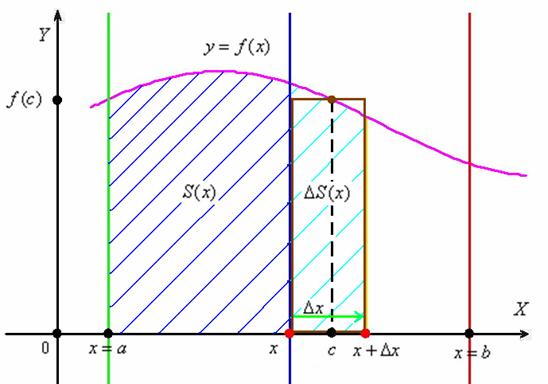
\includegraphics{img/471.jpeg}\\
Опр.
\[
  \lim_{max \Delta x\to 0}\sum_{i=1}^{n}f(\xi_i)\Delta x =\int_{a}^{b}f\left(x\right)dx   
\]
$ f(x) $ называется интегрируемой функцией на данном отрезке

\begin{mdframed}[backgroundcolor=blue!20] 
        Теорема 1:\\
        всякое  интегрируемая на отрезке функция ограниченна на этом отрезке(необходимое но недостаточное)\\

        Теорема 2(Рассы интегрируемых функций)\\
        Всякая непрерывная на отрезке функция интегрируема на этом отрезке\\
        Кусочно-непрерывные функции(функции имеющие на отрезке конечное число точек разрыва первого рода) также являются интегрируемы\\

     \end{mdframed}

Основные свойства определенного интеграла:\\
1)$ \int_{a}^{b}dx = b - a  $ \\
2)$ \int_{a}^{a}f\left(x\right)dx = 0 $ \\
3) $ \int_{a}^{b}f\left(x\right)dx = - \int_{b}^{a}f\left(x\right)dx   $ \\
4)линейнойсть: $ \int_{a}^{b}\left(f(x) + \lambda g(x)\right)dx= \int_{a}^{b}\left(f(x)\right)dx + \lambda \int_{a}^{b}\left(g(x)\right)dx    $ \\
5)аддитивность: $ \int_{a}^{c}f\left(x\right)dx + \int_{c}^{b}f\left(x\right)dx = \int_{a}^{b}f\left(x\right)dx  $ \\ 
6)монотонность: $ f(x),g(x) \quad [a,b] \quad f(x) \leq g(x) $\\
$ \int_{a}^{b}f\left(x\right)dx \leq \int_{a}^{b}g\left(x\right)dx $  \\
7)оценка модуля: $ \left| \int_{a}^{b}f\left(x\right)dx\right| \leq \int_{a}^{b}f\left(x\right)dx   $\\
\begin{mdframed}[backgroundcolor=blue!20] 
        Теорема о среднем(для непрерывных функций):\\
        $ f(x) $ непрерывна на AB:$ \exists \xi \in [a,b] $:
        \[
            \int_{a}^{b}f\left(x\right)dx= f(\xi)(b\cdot a) 
          \]  
     \end{mdframed}



\subsection{Параграф. Интеграл с переменным верхним пределом}
Предворительно заметим:\\
1) Определенный интеграл не зависит какой буквой обозначается переменная интегрирования\\
2) Если функция интегрируема на отрезке, то точка она будет интегрируема на внутренних отрезках\\

Интеграл с переменным верхним пределом:\\
\[
  \Phi (x) = \int_{a}^{x}\left(f(t)\right)dt 
\]
св $ \Phi (x) $ :\\
1) непрерывна\\
2) дифференциируема\\
3) 

\subsection{Параграф. Формула Ньютона-Лейбница}
Функция непрерывна на данном отрезке.
\[
  \int_{a}^{b}\left(f(x)\right)dx = f(x) |_a^b = F(b) - F(a)
\]

\subsection{Параграф. Замена переменной в определенном интеграле и формула интегрирования по-частям}
$ x = \phi(t) $ непрерывно дифференциируема. $ a = \phi(\alpha ),b = \phi(\beta ) $. Определена непредельно сложная функция $ f(\phi(t)) $. Тогда справедливо:
\begin{align*}
    \int_{a}^{b}\left(f(x)\right)dx = \begin{vmatrix}
    x = \phi(t)\\ dx = \phi'(t)dt
  \end{vmatrix}= \int_{\alpha }^{\beta }f(\phi(t))\phi'(t)dt 
  \end{align*}

Формула интегрирования по-частям:\\
\[
  \int_{a}^{b}\left(u\right)dv = \left (uv)\right|_a^b - \int_{a}^{b}\left(v\right)du  
\]

\subsection{Параграф. Несобственные интегралы}
1) Несобственные интегралы от непрерывных функций на бесконечном промежутке\\
\[
  \int_{a}^{+inf}\left(f(x)\right)dx = \lim_{b\to 0}  \int_{a}^{b}\left(f(x)\right)dx 
\]
св:\\
1. $ 0\leq f(x)\leq g(x),\forall x \geq a $\\
a) $ \int_{a}^{+inf}\left(g(x)\right)dx  $ - сходится, то и сходится интеграл меньшей функции.\\
b) $ \int_{a}^{+inf}\left(f(x)\right)dx  $ - расходится, то и расходится интеграл от большей функции\\
2. $ \int_{a}^{+inf}|f\left(x\right)|dx  $ - сходится, то и интеграл от самой функции сходится(в этом случае интеграл называется абсолютно-сходящимся)\\

2) Несобственный интегралы от неограниченной функции на конечном промежутке\\
Неограничена в окресности точки b: [a,b)\\
\[
   \int_{a}^{b}f\left(x\right)dx = \lim_{ \epsilon   \to 0} \int_{a}^{b}f\left(x\right)dx  
 \] 
\subsection{Параграф. Геометрические приложения определенного интеграла}
1. Площадь плоской фигуры\\
\[
  \int_{a}^{b}f\left(x\right)dx 
\]
2. Объемы тела вращения\\
\[
  V = \int_{a}^{b}S\left(x\right)dx 
\]
S(x) -- площадь сечения\\\\
3. Длина дуги прямой\\
\[
  l = \int_{a}^{b}\left(\sqrt[]{1+(y'(x))^2}\right)dx 
\]
если параметрически:
\[
  x = x(t) \quad and \quad  y = y(t) \quad l = \int_{a}^{b}\left(\sqrt[]{(x'(t))^2 + (y'(t))^2}\right)dt 
\]
полярные координаты:
\[
  l = \int_{a}^{b}\left(\sqrt[]{(r(\phi))^2 + (r'(\phi))^2}\right)d\phi 
\]

\section{Глава. Числовые и функциональные ряды}
\subsection{Параграф. Сходящиеся числовые ряды}
-- числовым рядомм называется выражение:\\
\[
   \sum_{n=1}^{} a_n = a_1+a_2+\ldots+a_n+\ldots  
 \] 

$ S_n $ -- сумма первых n слагаемых \\

Числовой ряд называется сходящимся если существует конечный предел последовательности его частичных сумм при n стремящимся к бесконечности
\[
  S = \lim_{n\to 0} S_n
\]
Если такой предел не существует или бесконечен, то ряд называется расходящимся.\\

Необходимы признак сходимости ряда:\\
Если числовой ряд сходится, то предел равен нулю\\
Следствие:\\
Если предел не равен нулю то ряд расходится\\

\subsection{Параграф.Сходимость знакоположительных рядов}
\[
  \sum_{n=1}^{}a_n \quad a_n > 0  
\]
\begin{mdframed}[backgroundcolor=blue!20] 
       Теорема 1(признак сравнения)\\
       Пусть данны два знакоположительных ряда, и $ a_n \leq b_n $, тогда справедливо утверждение:\\
       1) если сходится второй, то сходится и первый\\
       2) если первый расходится, то и второй расходится\\ 
    \end{mdframed}





\newpage
\subsection*{Литература}
Кудрявцев А.Д Курс математического анализа\\
Фихтенгольц Г.М Основы математического анализа\\
Демидович Б.П Сборник задач и упражнений по математическому анализу\\

\end{document}